% Capítulo 2
\chapter{Fundamentação Teórica} \label{ch:fundamentacao-teorica}

% TODO Revisar para ajustes a mudanças no capítulo.
Este capítulo apresenta uma visão geral das bases teóricas que fundamentam as
proposições  e  discussões  contidas  nesta  dissertação,  tais  como  Plataforma
Android (Seção \ref{sec:plataforma-android}), com ênfase no suporte a múltiplas
versões da API; Padrões de Projeto (Seção  \ref{sec:padroes-de-projeto}), 
destacando os que foram identificados nesta pesquisa; um Framework para Comparação
de Técnicas de Implementação de Variabilidades (Seção \ref{sec:framework}); e,
por fim, uma Taxonomia dos Componentes da API Android (Seção \ref{sec:taxonomia}). 

\section{Plataforma Android} \label{sec:plataforma-android}

Android é um sistema operacional projetado para dispositivos móveis, incluindo
celulares, \textit{tablets}, relógios inteligentes, televisões e até carros.
O sistema operacional é baseado no núcleo Linux, interagindo com o \textit{hardware}
em baixo nível e fornecendo conjuntos de API para acesso a serviços e demais
funções\cite{Lecheta2015}, apresentando uma arquitetura em camadas, conforme
figura \ref{fig:android_camadas}. É sobre essa API que os desenvolvedores irão
criar suas aplicações, portanto, mudanças nela afetarão diretamente as aplicações.

\begin{figure}[h]
	\centering
  	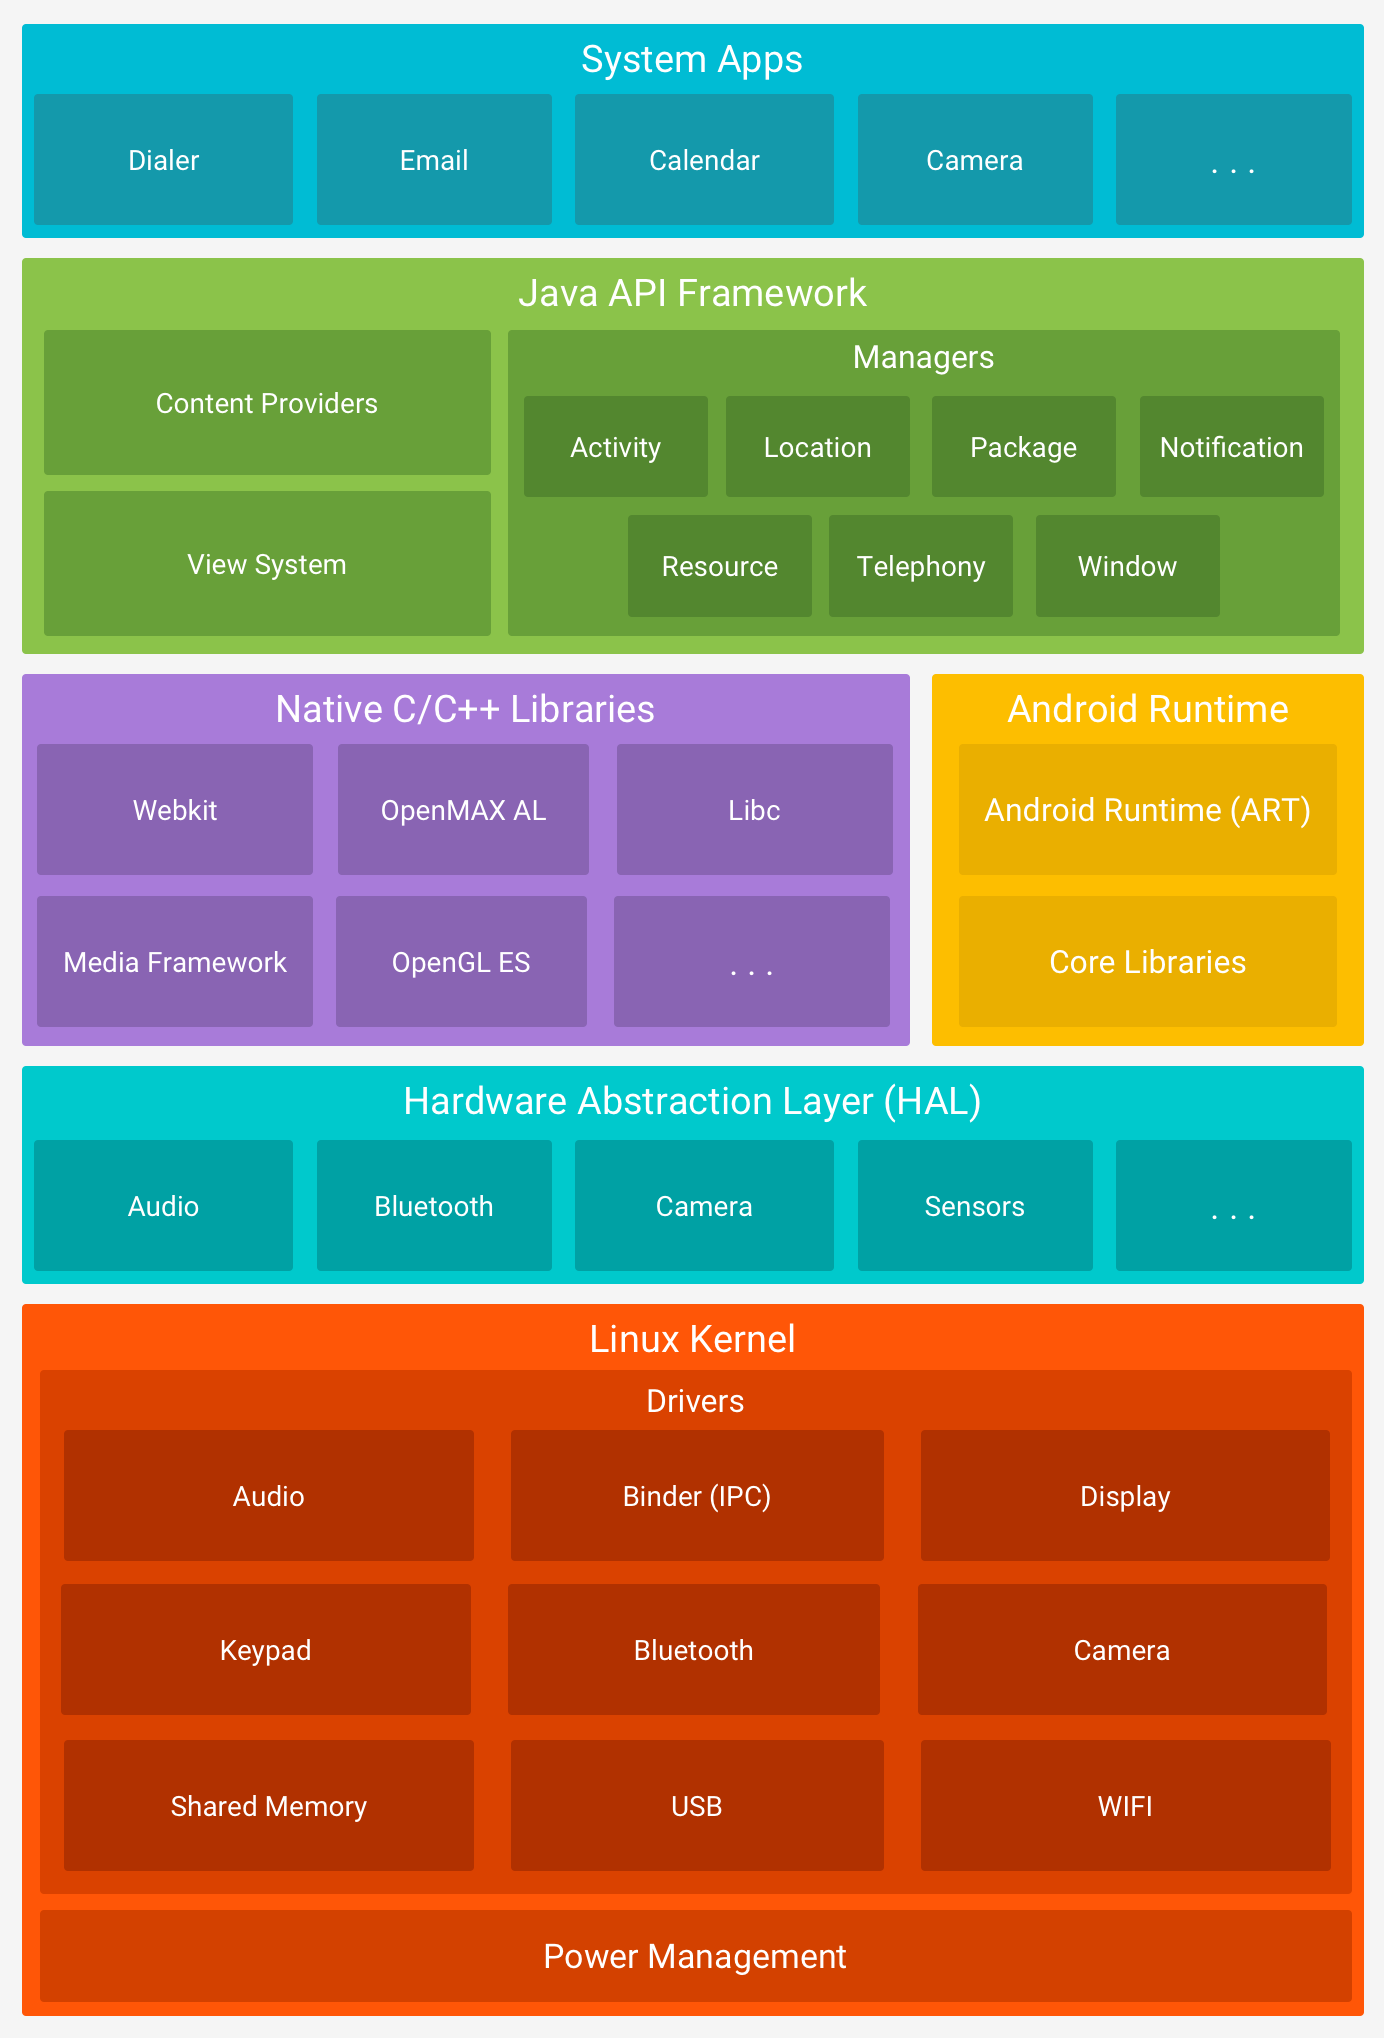
\includegraphics[scale=0.2]{imagens/android-stack_2x.png}
  	\textsf{\caption{Arquitetura em Camadas da Plataforma Android.}
  	        {Fonte: Guia Android \cite{Architecture2016}.\label{fig:android_camadas}}}
\end{figure}

Aplicações Android são desenvolvidas em cima da camada \textit{Java API Framework},
utilizando essa linguagem de programação, e são executadas em uma máquina virtual
chamada
\abrv[DVM -- \textit{Dalvik Virtual Machine}]
{DVM}(\textit{Dalvik Virtual Machine}). 
Essa máquina virtual é uma tecnologia \textit{open-source} e diferencia-se da
\abrv[JVM -- \textit{Java Virtual Machine}]
{JVM}(\textit{Java Virtual Machine}),
que é baseada em pilhas, por possuir uma arquitetura baseada em registros. Essa
arquitetura permite a DVM ser executada com pouca memória, além de possuir seu
próprio \textit{bytecode}.

\subsection{Loja de Aplicativos} \label{subsec:loja-aplicativos}

Usuários podem instalar novos aplicativos diretamente a partir de arquivos 
\abrv[APK -- \textit{Android Package}]
{APK}(\textit{Android Package})
ou obtê-los de lojas de aplicativos. A principal delas é a Google
Play\footnote{https://play.google.com}, mas outras também estão disponíveis, como
Amazon Appstore\footnote{https://www.amazon.com/b/ref=nav\_shopall\_adr\_banjo?ie=UTF8\&node=11350978011}.
Na Google Play, estão disponíveis mais de 2,2 milhões de aplicativos \cite{Statista2016}.

\subsection{Desenvolvimento de Aplicativos}
\label{subsec:desenvolvimento-aplicativos}

Para criar uma aplicação Android são utilizados Android Software Development Kit
\abrv[SDK -- \textit{Android Software Development}]
(SDK),
a linguagem de programação Java e a linguagem de marcação
\abrv[XML -- \textit{Extensible Markup Language}]
{XML}(\textit{Extensible Markup Language}).
O ambiente de desenvolvimento oficial é o Android Studio\cite{Studio2016}, que
oferece de forma integrada diversas ferramentas para a criação de aplicações e
recursos como edição de código, depuração, sistema flexível de compilação, emuladores,
ferramentas de desempenho e análise de código, como o Android Lint \cite{Lint2016},
que foi utilizado neste trabalho e será mais detalhado na seção \ref{subsec:android-lint}.

Uma aplicação Android consiste dos seguintes componentes \cite{Fundamental2016}:
\begin{itemize}
    \item Atividade: uma atividade é a classe onde a inferface com o usuário é
    implementada. Atividades também podem ser consideradas as tarefas que um
    usuários pode fazer em uma tela. Por exemplo, enviar um email pode ser feito
    em um atividade, enquanto escrever o email pode ser feito em outra atividade.
    Cada aplicação tem uma atividade especial chamada “atividade principal”, que
    é o ponto de entrada da aplicação \cite{Atividade2016}. Uma aplicação contém
    múltiplas atividades que podem iniciar umas às outras para diferentes ações.
    Quando uma atividade inicia ela é colocada no topo de uma pilha chamada pilha
    de retorno. Quando o usuário pressiona o botão de voltar, a atividade atual
    é removida da pilha e a atividade anterior é exibida para o usuário. Normalmente,
    atividade removidas da pilha são destruídas e coletadas pelo coletor de lixo.
    Gerenciamento do ciclo de vida de uma aplicação é uma importante tarefa do
    desenvolvimento. Uma instância de uma atividade tem seu estado alterado entre
    diferentes possibilidades, que são:
    \begin{itemize}
        \item Ativa: atividade está na frente da tela;
        \item Pausada: atividade perdeu o foco, mas ainda é visível;
        \item Parada: atividade está completamente oculta por outra atividade;
        \item Destruída: quando parada ou pausada, o sistema encerra a atividade.
    \end{itemize}
    Para cada estado, o sistema chama uma série de métodos do ciclo de vida \cite{CicloVidaAtividade2016},
    apresentada na figura \ref{fig:activity_lifecycle}. O método “onCreate” é
    chamado quando a atividade é iniciada pela primeira vez, método “onStart” é
    chamado quando a atividade torna-se visível para o usuário, “onRestart” é
    chamado quando a atividade pausada mas não destruída é novamente iniciada,
    “onResume” é  chamado quando a atividade inicia a interação com o usuário,
    “onPause” é chamado quando o sistema inicia a atividade anterior, “onStop” é
    chamado quando a atividade não é mais visível, “onDestroy” é o método final
    chamado antes da atividade ser destruída pelo sistema.
    \begin{figure}[htb]
    	\centering
      	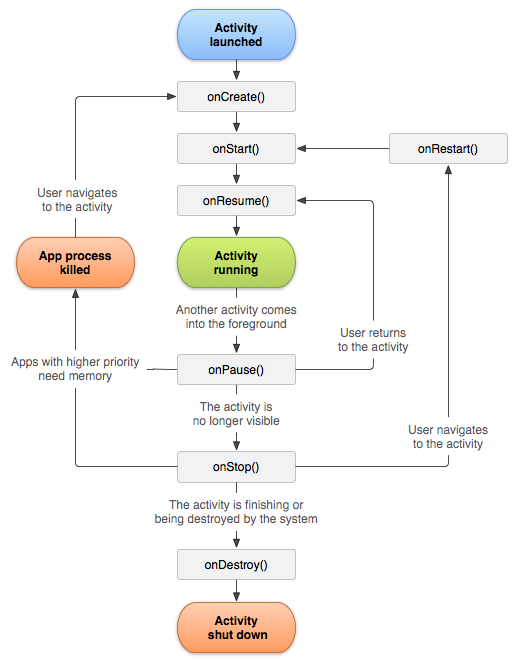
\includegraphics[scale=0.5]{imagens/activity_lifecycle.png}
      	\textsf{\caption{Ciclo de vida da atividade.}
      	        {Fonte: Guia Android \cite{CicloVidaAtividade2016}.\label{fig:activity_lifecycle}}
      	}
    \end{figure}
    \item Serviço: um serviço é um componente da aplicação que persiste por um
    longo tempo em \textit{background}, o que significa dizer que não tem uma
    interface com o usuário. Uma das mais importantes propriedade dos serviços é
    que eles podem executar em \textit{background} mesmo que o usuário alterne
    entre aplicações \cite{Servico2016};
    \item Provedor de conteúdo: provedores de conteúdo podem ser considerados como
    gerenciadores de acesso a servidores de dados para um conjunto estruturado de
    dados. Eles são a padronização para transmissão de dados entre processos \cite{Provedor2016}. 
    \item Receptor de mensagem: um receptor de mensagem é usado para executar uma
    aplicação para responder a eventos enviados para todo o dispositivo, tais como
    o recebimento de uma mensagem de texto ou notificação de baixa carga de
    bateria \cite{Receptor2016}.
\end{itemize}



\subsection{Suporte a múltiplas versões da API} \label{sec:suporte-multiversao}

Um aspecto chave no desenvolvimento de aplicações Android são as versões da API. 
Google disponibilizou a primeira versão do Android (Android 1.0, API 1) em setembro
de 2008, desde então uma nova versão da API é disponibilizada aproximadamente a
cada 3 meses. Nesse momento, a última versão disponibilizada é a 24. Para este
trabalho foram consideradas, por questões de padronização das análises, configuração
do ambiente de desenvolvimento e mercado, aplicações que usaram até a versão 23.

Apesar da rápida evolução do Android, a adoção das novas API’s é lenta e o mercado
consumidor é fragmentado em relação ao número de versões da API. O que obriga os
desenvolvedores de aplicações a tomarem decisões de projeto como usar as versões
mais recentes da API e deixar de lado um mercado consumidor que não usa determinada
API ou atender a esse mercado consumidor mas não usar as novidades da API mais recente.

Para auxiliar nessa decisão, o Google disponibiliza estatísticas de uso das versões
da API\cite{Dashboard2017}, conforme mostra a figura \ref{fig:platform_versions},
e mecanismos para o suporte a múltiplas versões. Ou seja, é possível atender um
usuário com baixa versão de API ao mesmo tempo que é possível usar recursos mais
modernos da plataforma. Tais mecanismos são apresentadas nas seções seguintes.

\begin{figure}[htb]
	\centering
  	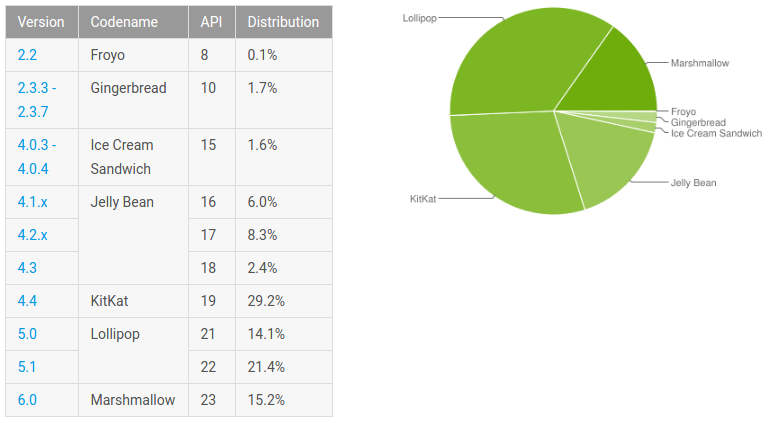
\includegraphics[scale=0.5]{imagens/platform_versions.png}
  	\textsf{\caption{Distribuição das versões da API do Android.}
  	        {Fonte: Android \cite{Dashboard2016}.\label{fig:platform_versions}}
  	}
\end{figure}

Embora 23 versões da API tenha sido lançadas, na figura \ref{fig:platform_versions}
são apresentadas somente 10 versões. Isso ocorre porque versões com uma distribuição
inferior a 0,1\% são omitidas. % TODO Acrescentar 
                                % Além disso, importante saber que 0,1%, embora
                                % pequeno em valores percentuais, representam XXX
                                % milhões de aparelhos. 
                                % (se achar a referencia que dizia isso.) 

% TODO Acrescentar algo sobre versão mínima e versão alvo

\subsubsection{Pacote de Compatibilidade} \label{subsec:pacote-compatibilidade}

Pacotes de compatibilidade \cite{SupportLibrary2017}, ou bibliotecas de suporte,
permitem que aplicações em execução sob versões antigas da plataforma utilizem
recursos que foram disponibilizadas em versões mais novas. Por exemplo, uma aplicação
instalada em um aparelho com API de nível 8 pode usar a API de fragmentos,
disponibilizada apenas no nível 11.

Esses pacotes são tradicionais arquivos JAR com classes, interfaces e outros
artefatos de recursos que poderão ser adicionados na aplicação. Assim, quando se
deseja usar a classe \texttt{Fragment}, por exemplo, em vez da importação ser da
API padrão do Android, como mostra a Figura \ref{fig:import_fragment_api},
deverá ser feita desse pacote que está junto da aplicação, como mostrado na Figura
\ref{fig:import_fragment_compat}.

\begin{figure}[htb]
	\centering
  	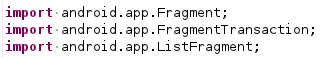
\includegraphics[scale=0.75]{imagens/import_fragment_api.png}
  	\textsf{\caption{Importando classes relacionadas a fragmentos da API padrão}
  	        \label{fig:import_fragment_api}
  	        }
\end{figure}


\begin{figure}[htb]
	\centering
  	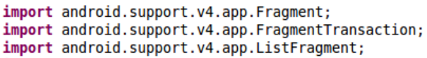
\includegraphics[scale=0.75]{imagens/import_fragment_compat.png}
  	\textsf{\caption{Importando classes relacionadas a fragmentos do pacote de compatibilidades}
  	        \label{fig:import_fragment_compat}
  	        }
\end{figure}

Como resultado, a aplicação será distribuída com uma experiência de uso mais consistente
através de um grande número de versões da plataforma.

\subsubsection{Re-implementação de recursos}
\label{subsec:reimplementacao-recursos}

Re-implementação de recursos ocorre quando se deseja um comportamento já provido
por versões mais recentes ou outra biblioteca, mas opta-se por re-implementar tal
recurso. Tal implementação pode ocorrer de três formas:

\begin{itemize}
    \item Re-implementação própria \cite{Base642016};
    \item Cópia do código-fonte da API padrão \cite{StackOverflow2016};
    \item Cópia do código-fonte de biblioteca de terceiro que implementa o recurso
    \cite{NineOldAndroids}.
\end{itemize}

Verificamos que 14 de 25 aplicações analisadas optaram por essa abordagem. Entre
elas, o aplicativo de mensagens Telegram ao re-implementar algumas classes relacionadas
a animações gráficas, quando poderia ter utilizado um pacote de compatibilidade
com o recurso pronto. A figura \ref{fig:telegram_diretorio_1} apresenta a estrutura
de pacotes do Telegram, com destaque para as classes que re-implementam o pacote
\texttt{android.animation} da plataforma, provento funcionalidades de animação
para a aplicação, mesmo em dispositivos com nível da API inferior a 11, quando
esse pacote foi disponibilizado.

\begin{figure}[htb]
	\centering
  	\frame{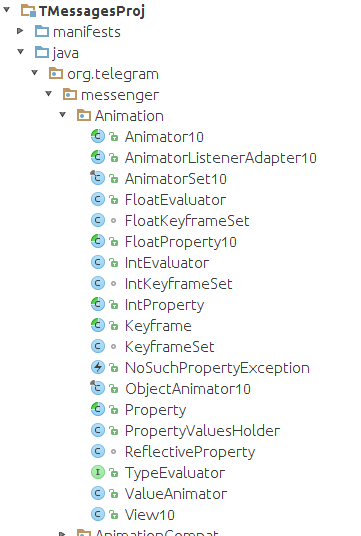
\includegraphics[scale=0.50]{imagens/telegram_diretorio_1.png}}
  	\textsf{\caption{Estrutura parcial de pacote do Telegram}.
  	        \label{fig:telegram_diretorio_1}
  	       }
\end{figure}

\subsubsection{Uso explícito da nova API}
\label{subsec:uso-explicito-nova-api}

Uso explícito da nova API ocorre quando é feita uma chamada a um novo recurso da
API, disponibilizado apenas em uma versão da API superior à mínima exigida para
execução da aplicação \cite{SupportDifferentVersions}. A figura \ref{fig:alert_android_studio}
apresenta um alerta do Android Studio indicando uma chamada para um método da API
nível 11, em uma aplicação que poderá ser instalada em qualquer aparelho com API
igual ou superior a nível 4.

\begin{figure}[htb]
	\centering
  	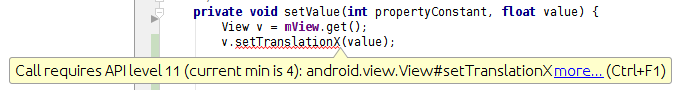
\includegraphics[scale=0.6]{imagens/alert_android_studio.png}
  	\textsf{\caption{Alerta do Android Studio sobre uso explícito da nova API}
  	    \label{fig:alert_android_studio}
  	    }
\end{figure}


Caso a chamada seja realmente feita durante a execução da aplicação, será lançada
uma exceção e a aplicação será interrompida, causado uma má experiência de uso.
Dessa forma, é necessário proteger tal chamada, fazendo com que ela só seja realmente
executada em ambientes seguros, no caso, em versões da API igual ou superior a 11.
As seções seguintes apresentam soluções de projeto que podem ser utilizadas para
proteger usos explícitos de novas API’s. 

\subsubsection{Execução condicional }
\label{sec:execucao-condicional}

\abrv[EC -- \textit{Execução Condicional}]
{Execução condicional} (EC) é um padrão para tratar variabilidades em granularidade
fina em linhas de produto de software \cite{Santos2012}. O padrão é composto por
4 elementos principais, ilustrados na Figura \ref{fig:execucao_condicional}:

\begin{itemize}
    \item Classes alvo: componentes do sistema onde ocorre a variabilidade acontece;
    \item Implementação da variabilidade: o código que representa a variabilidade,
    podendo ser um trecho diretamente na classe algo ou uma chamada para um componente
    que implementa a variabilidade; 
    \item Gerenciador da execução: é um elemento central do padrão, responsável
    por decidir qual implementação da variabilidade será executada;
    \item Repositório de parâmetros:  responsável por armazenar os valores dos
    parâmetros que será utilizado durante a execução condicional. É fundamental
    que a recuperação desses parâmetros não prejudique o desempenho das aplicações.
\end{itemize}

\begin{figure}[htb]
	\centering
  	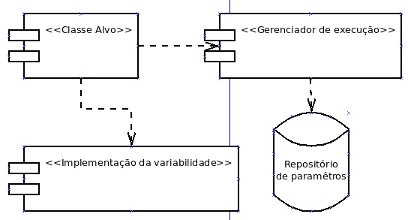
\includegraphics[scale=0.6]{imagens/execucao_condicional.png}
  	\textsf{\caption{Componentes principais do padrão execução condicional}
  	        {Adaptado de \cite{Santos2012}.\label{fig:execucao_condicional}}
  	       }
\end{figure}

Em aplicações Android, as classes alvo podem ser qualquer classe da aplicação.
Gerenciador de execução é uma instrução \texttt{if} que compara a versão da API
no dispositivo e uma versão cujo valor tem alguma importância para a variabilidade
em questão. Por exemplo, a versão em que um recurso surgiu ou mudou de comportamento.
Implementação da variabilidade costuma ser uma sequência de código para quando o
resultado dessa comparação é verdadeiro e outra sequência para quando ele é falso.
O repositório de parâmetros que armazenar os valores utilizados nesse contexto é 
a classe \texttt{android.os.Build}, que contém diversas informações sobre o sistema
instalado no aparelho, e suas classes aninhadas \texttt{VERSION} e \texttt{VERSION\_CODES}.
Em particular, a versão da API é obtida no atributo \texttt{Build.VERSION\_CODE.SDK\_INT},
já o outro valor da comparação é normalmente definida diretamente no código ou obtido de
\texttt{VERSION\_CODES}.

A figura \ref{fig:EC_in_cgeo2} apresenta um exemplo do uso de EC na aplicação C:geo.
A classe \texttt{AbstractDi alogFragment} % Esse espaço é gambiarra. Se ficar junto,
                                            % fica sem quebra de linha
é a classe alvo no padrão, do repositório
de parâmetros são obtidos os valores de \texttt{Build.VERSION.SDK\_INT} e
\texttt{Build.VERSION\_CODES.HONEYCOMB}, para serem utilizados na condição do
\texttt{if...else},  que faz o papel de gerenciador de execução. Também vemos
que existem duas implementação de variabilidade:
i) uma composta apenas por uma linha de código (\texttt{view.showContextMenu()}); e
ii) a outra composta por várias linhas e encapsulada no método
\texttt{showPopupHoneycomb(View view)}.

\begin{figure}[htb]
	\centering
  	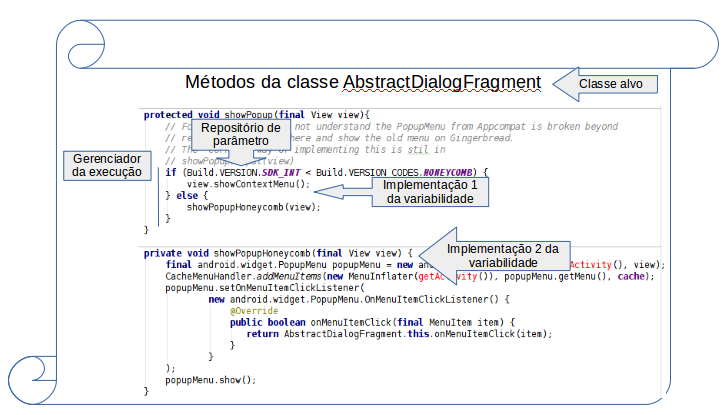
\includegraphics[scale=0.5]{imagens/EC_in_cgeo2.png}
  	\textsf{\caption{Exemplo do padrão EC no Cgeo}.\label{fig:EC_in_cgeo2}}
\end{figure}
 

Execução condicional é a forma indicada na documentação oficial
\cite{SupportDifferentVersions} para o suporte a múltiplas versões. Pode ser
utilizada em sua forma mais simples, como no exemplo acima, ou combinado com
padrões de projeto, como apresentado na seção \ref{sec:tecnicas_mais_comuns}.


\subsection{Android Lint}
\label{subsec:android-lint}

Android Lint \cite{Lint2016} é uma ferramenta do ambiente oficial de desenvolvimento
de aplicações Android capaz de analisar o código-fonte de uma aplicação para identificar
problemas estruturais, sem a necessidade de executá-la ou mesmo escrever testes.

Usos explícitos da nova API, portanto chamadas a elementos que não estão presentes
na versão mínima de API exigida pela aplicação, são exemplos de problemas estruturais,
podendo levar a falhas na execução, seja algum comportamento inesperado ou até
mesmo interrupção da aplicação. Existem duas centenas de verificações, também
chamadas de regras, feitas pelo Lint \cite{LintChecks}. Duas delas verificam por
acesso a elementos adicionados à API em versões superiores à versão mínima exigida
pela aplicação: InlinedApi e NewApi.

InlinedApi verifica por acessos a constantes. Durante o \textit{build} da aplicação os
valores dessas constantes serão copiados para os arquivos das classes que as
referenciam, o que significa dizer que os valores sempre estarão disponíveis,
mesmo executando em dispositivos com API antigas. Em alguns casos não haverá
problemas, em outros isso pode resultar em interrupção da execução ou comportamento
incorreto. Dependerá do contexto, então os desenvolvedores deverão avaliar com cuidado
se o código poderá ser executado em qualquer situação ou não.

NewApi verifica por chamadas a métodos e referências a classes. Como chamadas a
métodos só podem ser resolvidas em tempo de execução, será lançada uma exceção do
tipo \texttt{java.lang.NoSuchMethodError}, ou similar, levando ao travamento da
aplicação, sempre que a chamada for feita em dispositivos com API antigas.

Dessa forma, nessa dissertação de mestrado focaremos apenas nas ocorrências de NewApi.


\section{Framework para Comparação de Técnicas de Implementação de Variabilidades}
\label{sec:framework}

As diversas versões de API existentes na plataforma Android, em um contexto de
engenharia de 
\abrv[LPS -- \textit{Linha de Produtos de Software}]
{linha de produtos de software} (LPS)
\cite{Clements2002}, são conhecidas como variabilidades. Existem diversas técnicas
para implementação de variabilidades, de forma que se faz necessários critérios
de comparação e seleção de qual utilizar em uma determinada situação. Alves \cite{Alves2007}
propôs um framework para comparação de tais técnicas. O framework é uma extensão
de outros trabalhos \cite{Gacek2001} \cite{Coplien1999}, cujos critérios de avaliação
e valores possíveis estão apresentados na Tabela \ref{tab:framework}.

\begin{table}[h]
  \caption{Framework para comparação de técnicas de implementação de variabilidades}
  \begin{tabular}{ | l | l |}
    \hline
    \textbf{Critério de avaliação} & \textbf{Valores possíveis}  \\ \hline
    Tipo de variabilidade & Positivo, negativo ou ambos  \\ \hline
    Variabilidade na estrutura & Oferece suporte ou não oferece suporte \\ \hline
    Variabilidade no comportamento & Oferece suporte ou não oferece suporte \\ \hline
    Granularidade & Fina ou grossa \\ \hline
    Tempo de ligação & Pré-processamento, compilação, implantação, execução \\ \hline
    Reusabilidade & Alta, média, ou baixa \\ \hline
    Legibilidade & Alta, média, ou baixa \\ \hline
    Desempenho & Alta, média, ou baixa \\ \hline
    Tamanho da aplicação & Alto impacto ou baixo impacto \\ \hline
    \begin{tabular}[c]{@{}l@{}}Suporte para implementação\\ modular de requisitos transversais\end{tabular}  & Oferece suporte ou não oferece suporte \\ \hline
  \end{tabular}
  \label{tab:framework}
\end{table}

\textbf{Tipo de variabilidade} indica a adição ou remoção de comportamento ou
estrutura quando comparada com uma implementação base. \textbf{Variabilidade na estrutura}
indica a possibilidade de estaticamente organizar elementos do programa,
como adição de métodos ou atributos em classes, enquanto \textbf{variabilidade no comportamento}
diz respeito a diferentes semânticas de execução. \textbf{Granularidade fina}
refere-se avariações em nível de métodos de classe, incluindo trechos no corpo
dos métodos, ao passo que \textbf{granularidade grossa} é uma variação em nível
de classes. \textbf{Tempo de ligação} indica o momento durante o desenvolvimento
em que as decisões acerca da variação tem que ser tomada, por exemplo,
uma variação pode ser tratada durante a compilação ou somente no momento da execução.

Outros parâmetros importantes para avaliação são \textbf{reusabilidade}, \textbf{legibilidade},
\textbf{tamanho da aplicação} e \textbf{desempenho}, esses dois últimos dizem
respeito a um produto executável da LPS.

Também é considerado o suporte para implementação modular de requisitos transversais.
Esse suporte é importante porque muitas variabilidades de LPS podem ser requisitos
transversais, como apontado por diversas pesquisas \cite{Gacek2001} \cite{Batory2004}
\cite{Liu2006} \cite{Lopez2005} \cite{mezini2004}.

\section{Padrões de Projeto}
\label{sec:padroes-de-projeto}

Padrões de projeto \cite{Gamma1994}  e técnicas
\abrv[OO -- \textit{Orientação a Objetos}]
{orientação a objetos} (OO)
-- polimorfismo, herança, composição, agregação/delegação -- são abordagens utilizadas
para implementação de variabilidades de uma forma geral. Padrões de projeto
identificam aspectos do sistema que podem variar e fornecem soluções para gerenciar
a variação. Técnicas de OO são utilizadas para a implementação dos padrões de
projeto \cite{Gacek2001}. Com efeito, há relatos do uso de tal abordagem em linhas
de produto de software Android \cite{Pavlic2013}. Essa seção apresenta alguns
padrões de projeto encontrados durante a análise das aplicações.

\subsection{Strategy}
\label{sec:strategy}

O padrão \textit{Strategy} tem como objetivo "definir uma família de algoritmos,
encapsular cada uma delas e torná-las intercambiáveis. \textit{Strategy} permite
que o algoritmo varie independentemente dos clientes que o utilizam" \cite{Gamma}.
A figura \ref{fig:strategy_simple} apresenta uma visão geral do padrão. \texttt{Context}
é o cliente que usa os serviços de classes (\texttt{Strategy 1} e \texttt{Strategy 2})
que encapsulam os algoritmos de implementação da interface \texttt{Strategy}. 

\begin{figure}[htb]
	\centering
  	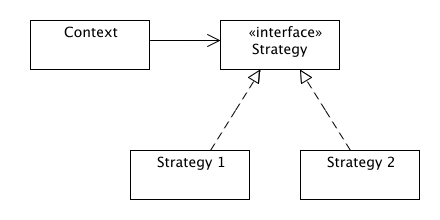
\includegraphics[scale=1]{imagens/strategy_simple.jpg}
  	\textsf{\caption{Visão geral do padrão Strategy}
  	        {Fonte: Best Practice Software Engineering (BPSE) \cite{StrategyPattern}}
  	        \label{fig:strategy_simple}}
\end{figure}

No contexto de versões da API, a interface \texttt{Strategy} pode conter um conjunto
de métodos que encapsulam serviços que mudam de uma versão para outra, e cada
implementação desse interface - \texttt{Strategy 1}, \texttt{Strategy 2} e assim
por diante - encapsula o comportamento desse serviço na versão respectiva da API.

Implementação de padrões de projeto podem variar entre si. Por exemplo, em um dos
aplicativos analisados, o  AnkiDroid, foi definida uma relação semântica de
dependência entre as implementações concretas da interface \texttt{Strategy}, que
no caso foi chamado de \texttt{Compat}. A interface \texttt{Strategy} contém todos
os métodos que encapsulam diferenças entre as diversas versões da API. A implementação concreta para a API de menor nível que a aplicação dará suporte, API de nível 10
neste caso, deve implementar a interface e escrever o código para os métodos referentes
à essa versão da API, deixando os métodos referentes às versões seguintes com corpo
vazio. A implementação concreta referente a próxima versão da API, nível 11 no caso,
deverá estender dessa classe e implementar o corpo do métodos relevante. E assim sucessivamente com as demais versões.

A Figura \ref{fig:strategy_ankidroid} apresenta um diagrama de classes simplificada
dessa estrutura. Nessa figura, também notamos a presença de um outro elemento: a
classe \texttt{CompatHelper}. Essa classe é responsável pela seleção e criação
das estratégias concretas. A Figura \ref{fig:strategy_compathelper} mostra o código
do método \texttt{CompatHelper}, onde a estratégia concreta é instanciada de acordo
com a versão do API do aparelho. Em outras variações do padrão, essas tarefas podem
ficar a cargo do próprio cliente ou em um método estático na interface \texttt{Compat},
que passará a ser uma classe abstrata. 

\begin{figure}[htb]
	\centering 
  	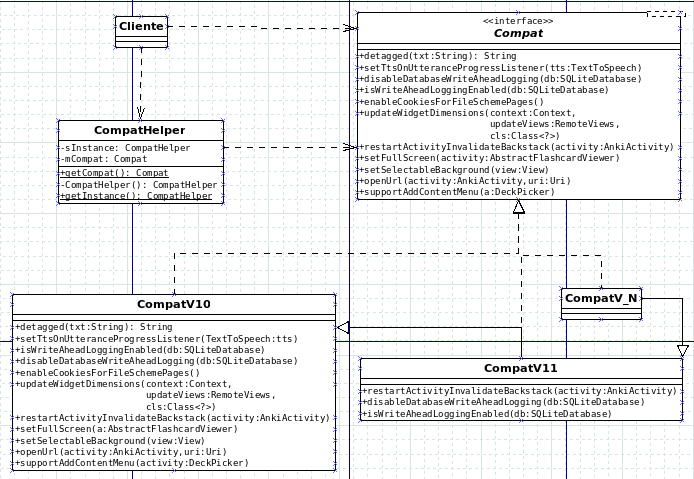
\includegraphics[scale=0.5]{imagens/strategy_ankidroid.png}
  	\textsf{\caption{Diagrama de classe da implementação do padrão Strategy na
  	                aplicação AnkiDroid}
  	        \label{fig:strategy_ankidroid}}
\end{figure}

\begin{figure}[htb]
	\centering % TODO alinhar caption no centro
  	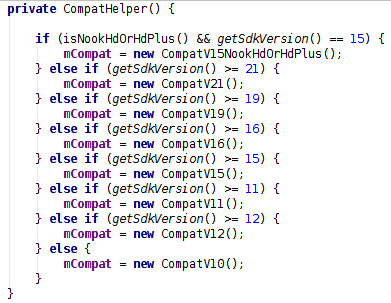
\includegraphics[scale=0.6]{imagens/strategy_compathelper.png}
    
  	\textsf{\caption{Trecho de código onde as implementações concretas são
  	                criadas de acordo com a nível da API no aparelho}
  	        \label{fig:strategy_compathelper}}
\end{figure}

\subsection{Template Method}
\label{sec:template-method}

O padrão \textit{Template Method} tem como objetivo "definir o esqueleto de um
algoritmo em um método, deixando alguns passos para subclasses" \cite{Gamma}.
A Figura \ref{fig:template_method} apresenta uma visão geral do padrão.
\texttt{AbstractClass} é a classe que contém o esqueleto do algoritmo, no método
\texttt{TemplateMethod()}. No esqueleto são feitas chamadas para métodos
(\texttt{PrimitiveOperation1} e \texttt{PrimitiveOperation2}) que são os passos
que deverão ser implementados pelas subclasses, representada por \texttt{ConcreteClass}.

\begin{figure}[htb]
	\centering 
  	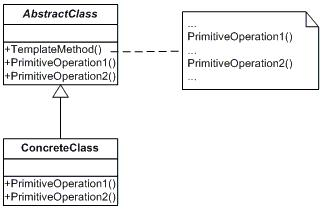
\includegraphics[scale=1]{imagens/template_method.jpg}
  	\textsf{\caption{Estrutura geral do padrão de projeto Template Method}
      	{Fonte: DoFactory \cite{TemplateMethod}}
  	        \label{fig:template_method}}
\end{figure}

No contexto de versões da API, os métodos abstratos são comportamentos que mudam
de uma versão para outra, já as classes concretas contém as implementações específicas necessárias para cada versão.

A aplicação que utilizou esse padrão de projeto, Wififixer, definiu como algoritmo
para tratar as diferenças entre as versões da API os seguintes passos:
\begin{itemize}
    \item Determinar o nível da API no aparelho;
    \item Executar o código específico do nível da API.
\end{itemize}

Assim, o algoritmo executa o passo \textbf{a} de forma fixa, implementado no
\textit{"template method"}, enquanto o passo \textbf{b} é delegado para a classe
concreta. A Figura \ref{fig:templatemethod_wififixer} mostra o código do método
\textit{template method} \texttt{getFile}, onde a parte fixa do algoritmo faz a
seleção da classe concreta de acordo com a versão da API e logo depois o método
abstrato \texttt{vgetLogFile} é chamado.

\begin{figure}[htb]
	\centering 
  	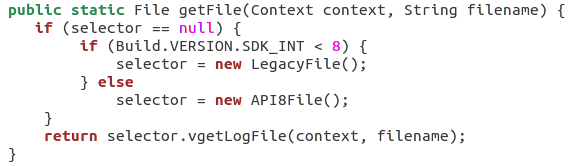
\includegraphics[scale=0.5]{imagens/templatemethod_wififixer}
  	\textsf{\caption{Exemplo de template method no aplicativo Wififixer}
  	        \label{fig:templatemethod_wififixer}}
\end{figure}

\section{Taxonomia dos Componentes da API} \label{sec:taxonomia}


